\documentclass{article}

%packages
\usepackage{graphicx}
\usepackage{tikz}
\usepackage[utf8]{inputenc}
\usepackage{amssymb}

\usepackage[T1]{fontenc}
\usepackage{mathabx}
\def\MCr{
	\multicolumn{1}{c}{
		\rule{-5pt}{0ex}$\stackrel{}{\curvearrowleft}$
		\rule{+20pt}{0ex}$\stackrel{}{\curvearrowright}$
	}
}
\def\MCe{\multicolumn{1}{c}{}}

\begin{document}

\usetikzlibrary{automata,arrows, positioning}
\renewcommand{\contentsname}{Tabla de contenidos}

\begin{titlepage}
	\begin{center}
		
\includegraphics{./images/escudo.jpg}
	\end{center}
	\centering
	{\scshape\LARGE Complutense de Madrid \par}
	\vspace{1cm}
	{\scshape\Large Práctica Programación Evolutiva.\par}
	\vspace{1.5cm}
	{\huge\bfseries Segunda práctica. \par}
	\vspace{2cm}
	{\Large\itshape Raúl Torrijos \& Lukas Häring\par}
	%{\large Grupo 9\par}
	\vfill
	\vfill

% Bottom of the page
	{\large \today\par}
\end{titlepage}

\tableofcontents


\section{Introducción}

\newpage

\section{Algoritmos Propios}

\subsection{Algoritmo de Mutación}
El algoritmo consiste en evaluar dos posibles mutaciones, estas mutaciones son las que se producen al intercambiar alguno de los vecinos más cercanos.
Algoritmo:
\begin{enumerate}
	\item Se genera un entero aleatorio desde $2$ hasta $n-2$, donde n es la cantidad de genes.
	\item Se realiza un intercambio del elemento que apunta este puntero con el vecino de la izquierda.
	\item Si su evaluación es mejor, intercambiamos. Por el contrario, lo dejamos como está.
	\item Teniendo en cuenta el cromosoma sin modificar, realizamos un intercambio con el vecino de la derecha.
	\item De la misma forma, si la evaluación es mejor, intercambiamos.
\end{enumerate}

Como vemos, el número aleatorio se elige entre $2$ y $n-2$. Esto es, claro está, que si intercambiamos el puntero fuera $1$, este cogería como vecinos $0$ y $2$, haciendo que pudiera mutar el gen inicial (Y eso no debe ocurrir).


\begin{tabular}{|l|*7{c|}}
	\MCe & \MCe & \MCe & \MCe & \MCr & \MCe & \MCe \\\hline
	Cromosoma 1 & $a_0$ & $\dots$ & $a_{k-1}$ & $a_{k}$ & $a_{k-1}$ & $\dots$ & $a_{n}$ \\\hline
\end{tabular}
\newline\newline
Donde $k\in \{2, \dots, n-2\}\subseteq\mathbb{N}$

%subsection{Función 1}
%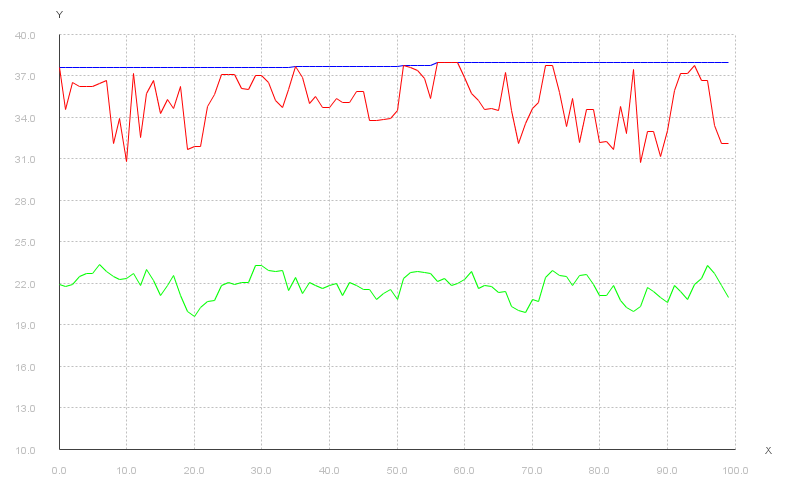
\includegraphics[scale=0.5]{./images/graph1_bin.png}
%En general, hemos observado que el grado de evolución global es mucho mayor cuando el elitismo está activado. La calidad media generacional se ve mejorada notablemente.




\end{document}
